\section{Lectura de los resultados}
\label{sec:resultados-lectura}

Con el umbral base de Google (0,65), el área de techos suma 222,17\,km$^2$ frente
a 221,13\,km$^2$ de Microsoft: los totales coinciden. La diferencia está en cómo se
reparten. Esta sección lee las cifras de \campo{resultados} desde tres ángulos: los
municipios, la sensibilidad al umbral y las subregiones.

\subsection{Municipio por municipio}

La figura~\ref{fig:res-dispersion} compara el área total de cada municipio en las
dos fuentes. Para 165 municipios con edificios de Google, la mayoría cae cerca de la
recta 1:1, así que ambas fuentes dan un orden de magnitud parecido. Los municipios
que se separan de la recta son pocos, y los que más se separan quedan por debajo de
Microsoft. Los más alejados son Sipí, López, Condoto, Carmen del Darién y Ricaurte.
En Sipí y López Google tiene casi nada: son municipios de cobertura baja, como se vio
en el mapa de control (sección~\ref{sec:eda}). Los cinco municipios sin edificios de
Google no aparecen en la figura.

\begin{figure}[H]
  \centering
  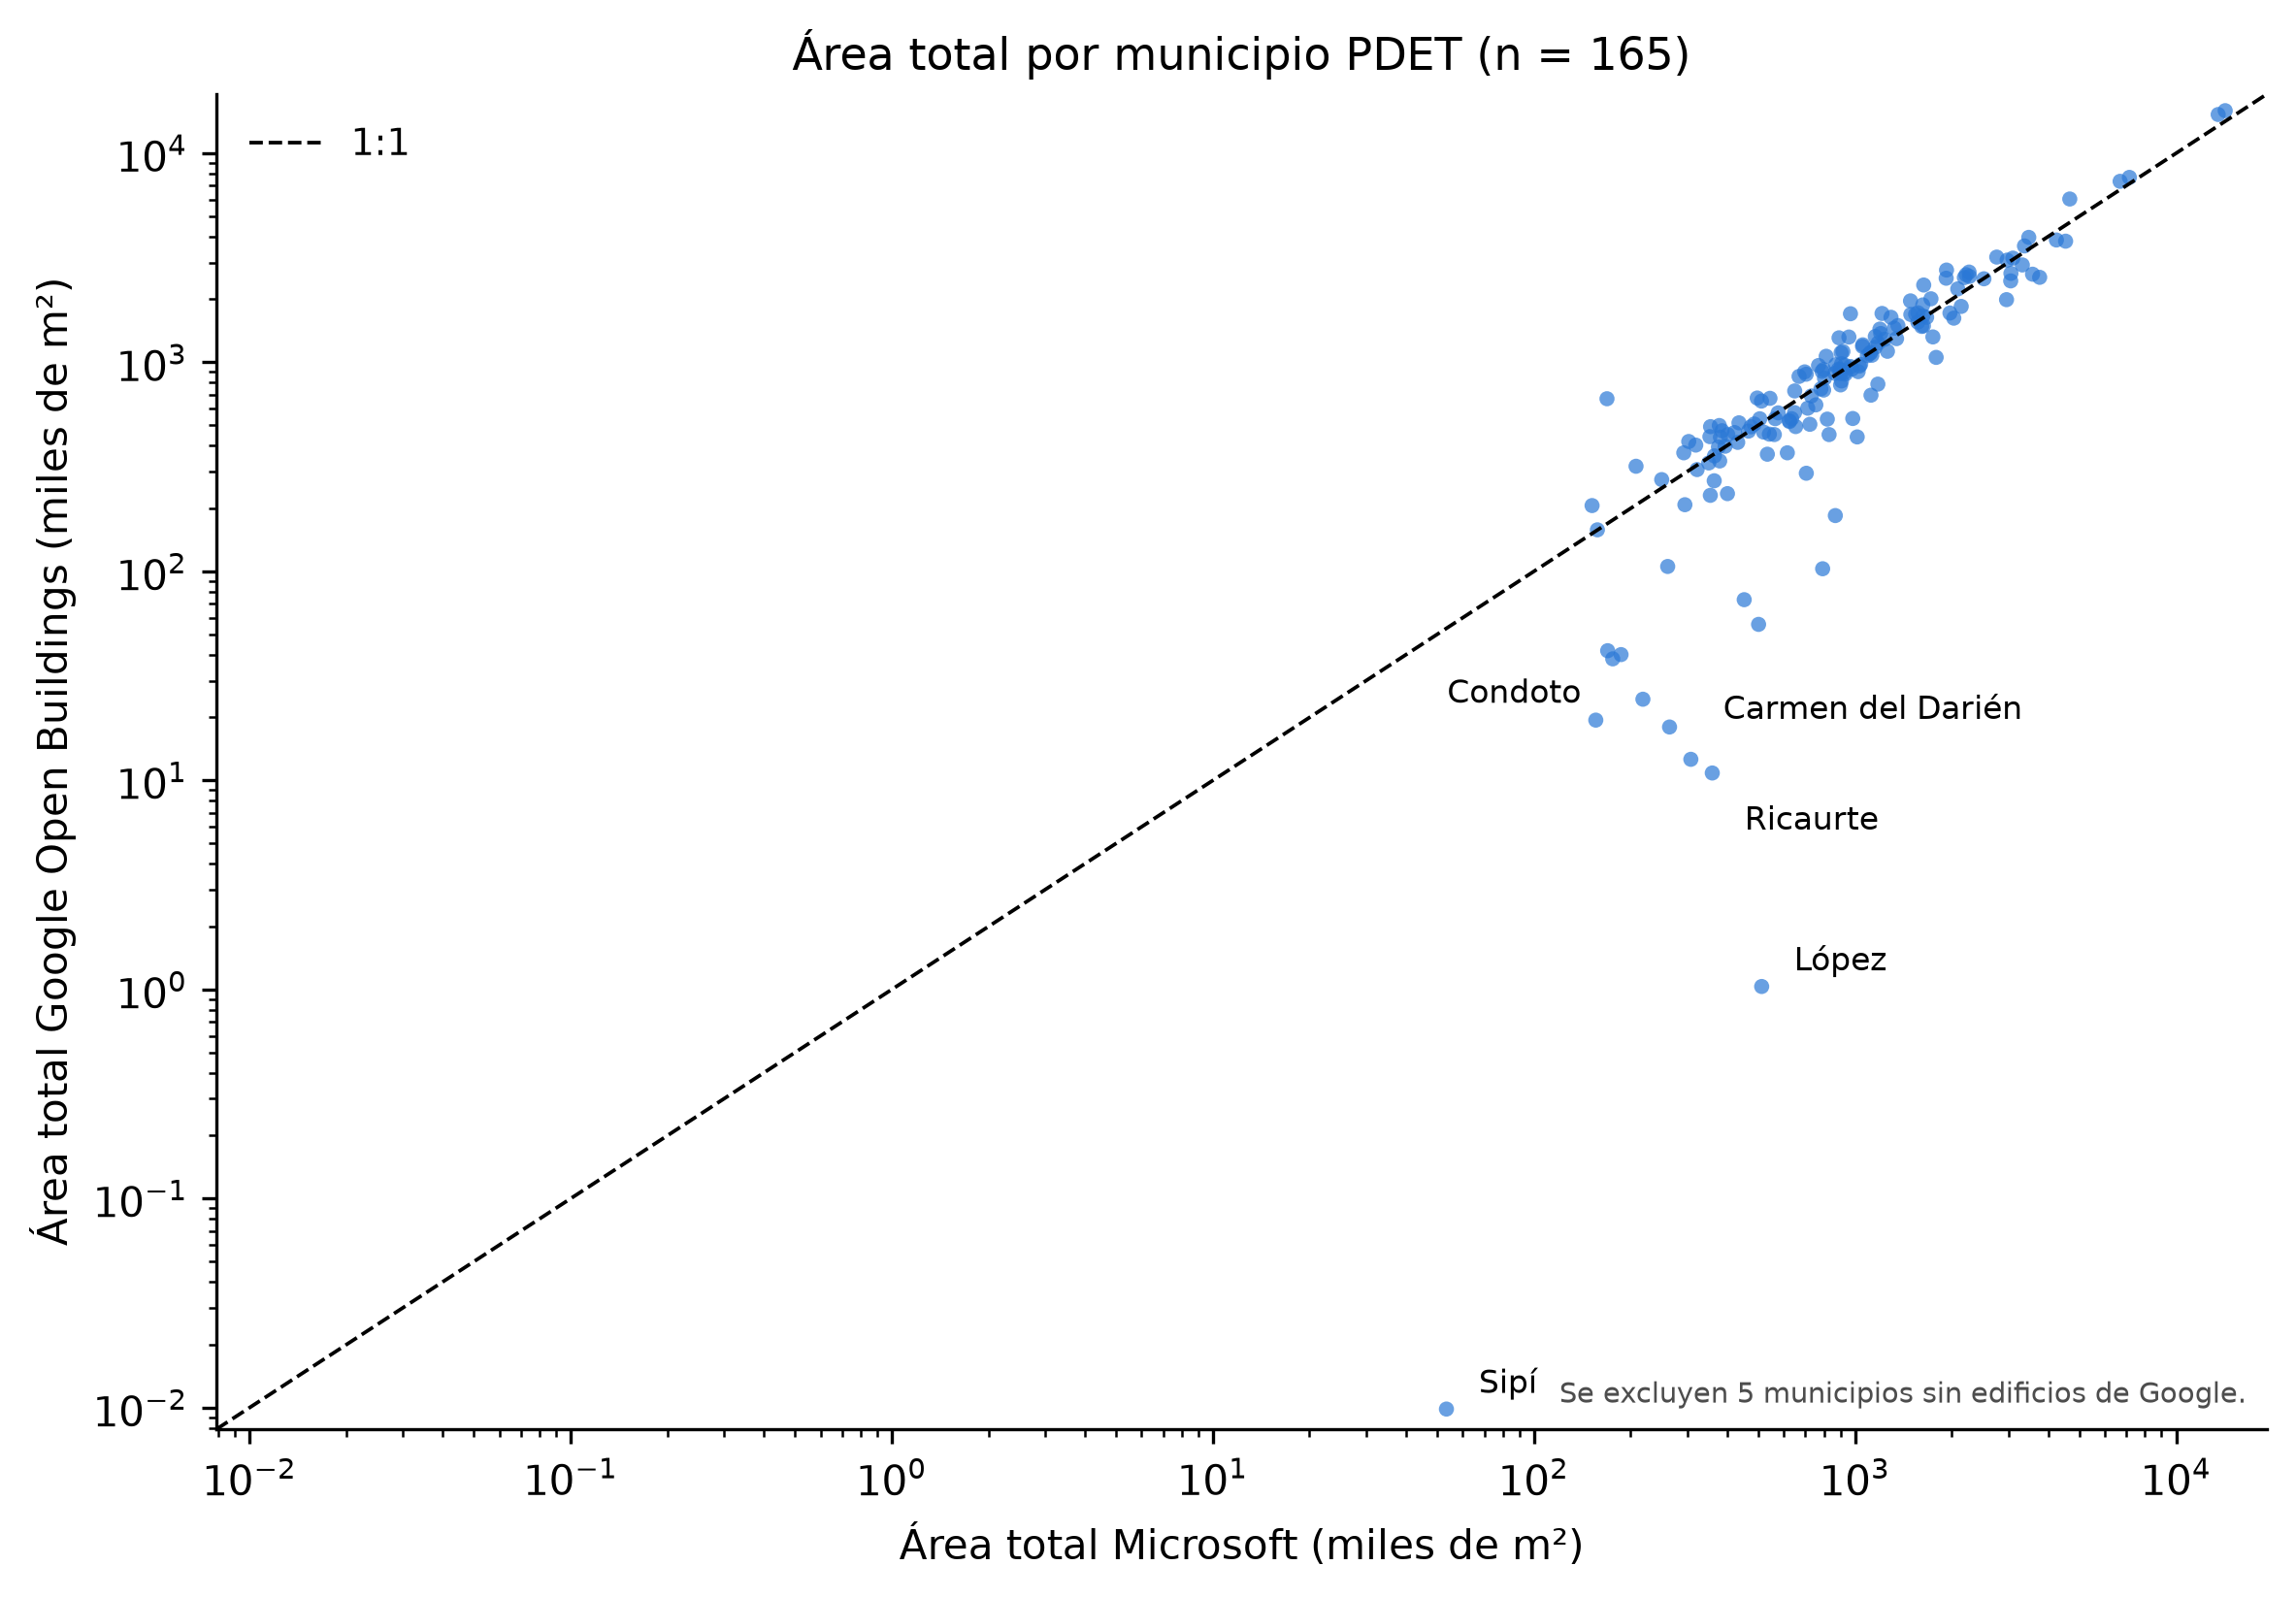
\includegraphics[width=0.85\textwidth,height=0.42\textheight,keepaspectratio]{img/res_dispersion_municipio.png}
  \caption{Área total por municipio PDET: Google con umbral 0,65 frente a Microsoft.
  La recta punteada es 1:1.}
  \label{fig:res-dispersion}
\end{figure}

\subsection{Sensibilidad al umbral}

Subir el umbral de confianza de Google quita edificios y área, como muestra la
figura~\ref{fig:res-sensibilidad} y la tabla~\ref{tab:sensibilidad}. Con 0,70 se
pierden 16\,\% de los edificios y 7\,\% del área; con 0,75, 35\,\% y 19\,\%. El top 15
de municipios por área se mantiene casi intacto: 15 de 15 con 0,70 y 14 de 15 con
0,75. Sin embargo, con 0,75 el área de Google (179,6\,km$^2$) queda por debajo de la
de Microsoft (221,1\,km$^2$), así que el umbral sí cambia la conclusión sobre qué
fuente tiene más techo. Por eso 0,65 se usa como escenario base y los otros dos se
reportan como sensibilidad.

\begin{figure}[H]
  \centering
  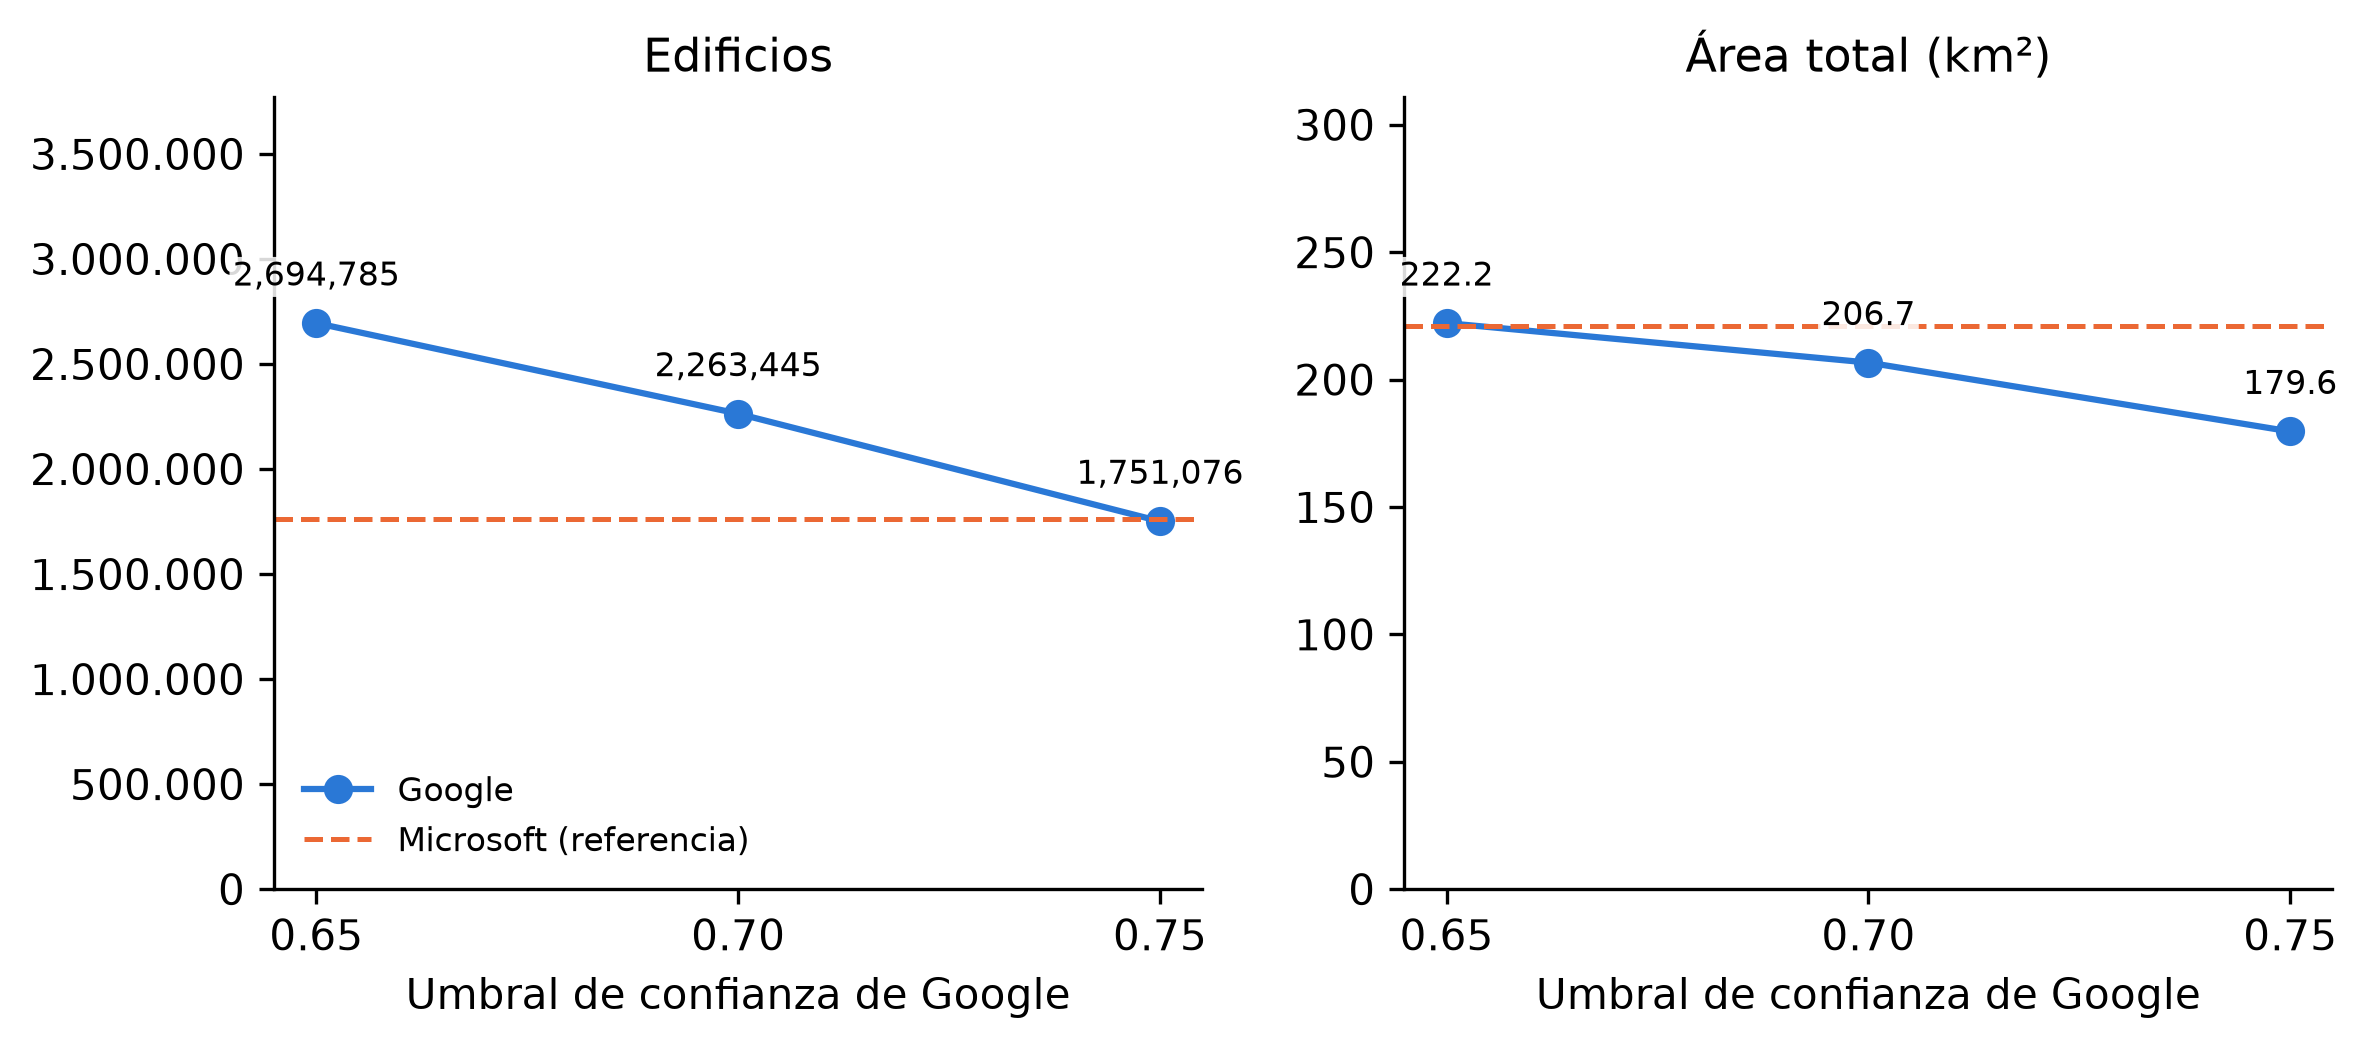
\includegraphics[width=0.9\textwidth,height=0.3\textheight,keepaspectratio]{img/res_sensibilidad_umbral.png}
  \caption{Edificios y área total de Google según el umbral de confianza, con
  Microsoft como referencia.}
  \label{fig:res-sensibilidad}
\end{figure}

\subsection{Subregiones}

La tabla~\ref{tab:subregion} muestra que la diferencia entre fuentes no es uniforme.
La columna $D$ es $(A_G - A_M)/(A_G + A_M)$: positiva cuando Google tiene más área.
En la Sierra Nevada - Perijá, Urabá Antioqueño y Montes de María, $D$ está entre
$+$0,07 y $+$0,09. En cambio, en el Chocó, el Sur del Tolima y el Pacífico y Frontera
Nariñense, $D$ está entre $-$0,21 y $-$0,33, es decir, Microsoft tiene más área. La
diferencia total es cero porque los excesos y los faltantes se compensan. Esto
confirma lo que muestra la figura: las fuentes coinciden en la escala regional, pero
no en las zonas de baja densidad del Pacífico y el sur, donde la cobertura de Google
es más débil.

\subsection{Lectura para el informe}

El total regional es robusto frente al umbral base: entre 0,65 y 0,70 el área baja 7\,\%,
y entre 0,65 y 0,75, 19\,\%. A nivel municipal la cifra sí depende de la fuente y del
umbral, sobre todo en el Pacífico y el Chocó, donde conviene reportar un rango y no
una sola cifra.
